\documentclass[11pt,a4paper]{article}
\usepackage[utf8]{inputenc}
\usepackage[T1]{fontenc}
\usepackage[brazil]{babel}
\usepackage{amsmath,amssymb,amsthm}
\usepackage{bm}
\usepackage{booktabs}
\usepackage{graphicx}
\usepackage{geometry}
\usepackage{hyperref}
\usepackage{float}

\geometry{margin=2.2cm}
\hypersetup{colorlinks=true, linkcolor=blue, urlcolor=blue}

\title{\textbf{Projeto Final — Álgebra Linear e Otimização para Machine Learning}\\
\large Relatório Técnico e Memorial de Cálculo Analítico}
\author{
Rafael Attilio Agricola (RA: \textit{249245}) \and
Guilherme De Godoi Monteiro (RA: \textit{237031}) \and
Lucas Peixoto Gonçalves (RA: \textit{233419})
}
\date{Instituto de Computação — UNICAMP \\ 2º Semestre de 2026}

\begin{document}
\maketitle

\setcounter{section}{1}
\section{Questão 2: Regressão Linear, Posto de Matrizes e Mínimos Quadrados Clássicos (OLS)}
% ==============================================================================

\subsection{Parte A: Formulação Matricial, Tipos de Sistemas e Posto}

\subsubsection*{A.1 e A.2. Matriz de Design, Posto e Teorema de Rouché--Capelli}
Adicionando a coluna unitária de \textit{bias} na primeira posição, o sistema $\mathbf{X}\mathbf{w} = \mathbf{y}$ é dado por:
\[
\mathbf{X} = \begin{bmatrix}
1 & 5{,}0 & 30{,}0 \\
1 & 7{,}0 & 38{,}0 \\
1 & 9{,}0 & 40{,}0 \\
1 & 3{,}5 & 19{,}0 \\
1 & 8{,}0 & 15{,}0 \\
1 & 2{,}0 & 35{,}0
\end{bmatrix} \in \mathbb{R}^{6 \times 3}, \qquad
\mathbf{y} = \begin{bmatrix} 2{,}5 \\ 3{,}8 \\ 4{,}2 \\ 1{,}9 \\ 4{,}5 \\ 1{,}2 \end{bmatrix} \in \mathbb{R}^6, \qquad
\mathbf{w} = \begin{bmatrix} w_0 \\ w_1 \\ w_2 \end{bmatrix} \in \mathbb{R}^3.
\]
Trata-se de um sistema \textbf{sobredeterminado}, pois possui $N = 6$ equações para $d + 1 = 3$ incógnitas. Escalonando a matriz aumentada $[\mathbf{X} \mid \mathbf{y}]$ por eliminação gaussiana ($L_i \leftarrow L_i - L_1$ para $i=2,\dots,6$, depois eliminando a segunda e terceira colunas):
\[
\left[\begin{array}{ccc|c}
1 & 5{,}0 & 30{,}0 & 2{,}5 \\
0 & 2{,}0 & 8{,}0 & 1{,}3 \\
0 & 4{,}0 & 10{,}0 & 1{,}7 \\
0 & -1{,}5 & -11{,}0 & -0{,}6 \\
0 & 3{,}0 & -15{,}0 & 2{,}0 \\
0 & -3{,}0 & 5{,}0 & -1{,}3
\end{array}\right]
\longrightarrow
\left[\begin{array}{ccc|c}
1 & 5{,}0 & 30{,}0 & 2{,}5 \\
0 & 2{,}0 & 8{,}0 & 1{,}3 \\
0 & 0 & -6{,}0 & -0{,}9 \\
0 & 0 & 0 & 1{,}125 \\
0 & 0 & 0 & 4{,}10 \\
0 & 0 & 0 & -1{,}90
\end{array}\right].
\]
O bloco $\mathbf{X}$ apresenta 3 pivôs não nulos, logo $\operatorname{rk}(\mathbf{X}) = 3$. A matriz aumentada $[\mathbf{X} \mid \mathbf{y}]$ apresenta um quarto pivô não nulo na última coluna, logo $\operatorname{rk}([\mathbf{X} \mid \mathbf{y}]) = 4$. Pelo \textbf{Teorema de Rouché--Capelli}, como $\operatorname{rk}(\mathbf{X}) \ne \operatorname{rk}([\mathbf{X} \mid \mathbf{y}])$, o sistema é \textbf{incompatível}. Geometricamente, $\mathbf{y}$ não pertence ao subespaço $\operatorname{Col}(\mathbf{X})$ de dimensão 3 em $\mathbb{R}^6$. Na prática, os preços observados trazem ruído e fatores não capturados por um modelo puramente linear em área e idade, impossibilitando que um plano passe exatamente pelos 6 pontos.

\subsubsection*{A.3. Multicolinearidade Exata}
Inserindo a coluna $x_3 = 2{,}5 x_1$, obtém-se $\tilde{\mathbf{X}} = [\mathbf{1} \quad \mathbf{x}_1 \quad \mathbf{x}_2 \quad 2{,}5\mathbf{x}_1] \in \mathbb{R}^{6 \times 4}$. Como a quarta coluna é múltiplo exato da segunda, o espaço-coluna não muda ($\operatorname{Col}(\tilde{\mathbf{X}}) = \operatorname{Col}(\mathbf{X})$), de modo que $\operatorname{rk}(\tilde{\mathbf{X}}) = 3$. Como $\operatorname{rk}(\tilde{\mathbf{X}}^T\tilde{\mathbf{X}}) = \operatorname{rk}(\tilde{\mathbf{X}}) = 3 < 4$, a matriz de Gram $4 \times 4$ torna-se singular (posto deficiente).

Esse fenômeno é a \textbf{multicolinearidade exata}: existe um vetor não nulo $\mathbf{v} = [0,\; -2{,}5,\; 0,\; 1]^T \in \mathcal{N}(\tilde{\mathbf{X}})$ tal que $\tilde{\mathbf{X}}\mathbf{v} = \mathbf{0}$. Assim, se $\hat{\mathbf{w}}^*$ resolve as equações normais, qualquer $\hat{\mathbf{w}}^* + \alpha\mathbf{v}$ ($\alpha \in \mathbb{R}$) também é solução, destruindo a unicidade dos parâmetros. Contudo, as previsões permanecem \textbf{únicas}, pois:
\[
\hat{\mathbf{y}} = \tilde{\mathbf{X}}(\hat{\mathbf{w}}^* + \alpha\mathbf{v}) = \tilde{\mathbf{X}}\hat{\mathbf{w}}^* + \alpha(\tilde{\mathbf{X}}\mathbf{v}) = \tilde{\mathbf{X}}\hat{\mathbf{w}}^*,
\]
que é a projeção ortogonal única de $\mathbf{y}$ sobre $\operatorname{Col}(\tilde{\mathbf{X}})$.

\subsection{Parte B: Resolução por Mínimos Quadrados e Interpretação}

\subsubsection*{B.1. Equações Normais e Eliminação Gaussiana}
Calculando $\mathbf{X}^T\mathbf{X}$ e $\mathbf{X}^T\mathbf{y}$ diretamente sobre $\mathcal{D}$:
\[
\mathbf{X}^T\mathbf{X} = \begin{bmatrix}
6{,}0 & 34{,}5 & 177{,}0 \\
34{,}5 & 235{,}25 & 1032{,}5 \\
177{,}0 & 1032{,}5 & 5755{,}0
\end{bmatrix}, \qquad
\mathbf{X}^T\mathbf{y} = \begin{bmatrix} 18{,}1 \\ 121{,}95 \\ 533{,}0 \end{bmatrix}.
\]
Resolvendo $\mathbf{X}^T\mathbf{X}\hat{\mathbf{w}} = \mathbf{X}^T\mathbf{y}$ por eliminação gaussiana:
\begin{enumerate}
    \item Subtraindo $\frac{34{,}5}{6} = 5{,}75$ vezes $L_1$ de $L_2$ e $\frac{177}{6} = 29{,}5$ vezes $L_1$ de $L_3$:
    \[
    \left[\begin{array}{ccc|c}
    6{,}0 & 34{,}5 & 177{,}0 & 18{,}1 \\
    0 & 36{,}875 & 14{,}75 & 17{,}875 \\
    0 & 14{,}75 & 533{,}5 & -0{,}95
    \end{array}\right].
    \]
    \item Subtraindo $\frac{14{,}75}{36{,}875} = 0{,}4$ vezes $L_2$ de $L_3$:
    \[
    \left[\begin{array}{ccc|c}
    6{,}0 & 34{,}5 & 177{,}0 & 18{,}1 \\
    0 & 36{,}875 & 14{,}75 & 17{,}875 \\
    0 & 0 & 527{,}6 & -8{,}10
    \end{array}\right].
    \]
    \item Por retrosubstituição:
    \[
    \hat{w}_2 = \frac{-8{,}10}{527{,}6} \approx -0{,}015353, \quad
    \hat{w}_1 = \frac{17{,}875 - 14{,}75\hat{w}_2}{36{,}875} \approx 0{,}490887, \quad
    \hat{w}_0 = \frac{18{,}1 - 34{,}5\hat{w}_1 - 177\hat{w}_2}{6} \approx 0{,}646968.
    \]
\end{enumerate}
Logo, $\hat{\mathbf{w}} \approx [0{,}646968,\; 0{,}490887,\; -0{,}015353]^T$, resultado idêntico ao obtido em Python via eliminação gaussiana manual, \texttt{np.linalg.solve} e \texttt{np.linalg.lstsq}.

\subsubsection*{B.2. Ortogonalidade do Resíduo e Interpretação Geométrica}
Seja $\hat{\mathbf{e}} = \mathbf{y} - \mathbf{X}\hat{\mathbf{w}}$. Multiplicando à esquerda por $\mathbf{X}^T$ e usando as Equações Normais:
\[
\mathbf{X}^T\hat{\mathbf{e}} = \mathbf{X}^T(\mathbf{y} - \mathbf{X}\hat{\mathbf{w}}) = \mathbf{X}^T\mathbf{y} - \mathbf{X}^T\mathbf{X}\hat{\mathbf{w}} = \mathbf{0}.
\]
Ou seja, $\hat{\mathbf{e}}$ é ortogonal a todas as colunas de $\mathbf{X}$ ($\hat{\mathbf{e}} \in \operatorname{Col}(\mathbf{X})^\perp$). Para qualquer outro vetor de pesos $\mathbf{w} \in \mathbb{R}^3$, tem-se $\mathbf{X}(\hat{\mathbf{w}} - \mathbf{w}) \in \operatorname{Col}(\mathbf{X})$, logo $\langle \hat{\mathbf{e}}, \mathbf{X}(\hat{\mathbf{w}} - \mathbf{w})\rangle = 0$. Pelo Teorema de Pitágoras:
\[
\|\mathbf{y} - \mathbf{X}\mathbf{w}\|_2^2 = \|\hat{\mathbf{e}} + \mathbf{X}(\hat{\mathbf{w}} - \mathbf{w})\|_2^2 = \|\hat{\mathbf{e}}\|_2^2 + \|\mathbf{X}(\hat{\mathbf{w}} - \mathbf{w})\|_2^2 \ge \|\hat{\mathbf{e}}\|_2^2,
\]
mostrando que a projeção ortogonal $\hat{\mathbf{y}} = \mathbf{X}\hat{\mathbf{w}}$ realiza a menor distância euclidiana até $\mathbf{y}$. Na validação em \texttt{numpy}, $\|\mathbf{X}^T\hat{\mathbf{e}}\|_\infty \approx 5{,}84 \times 10^{-14} < 10^{-10}$.

\subsubsection*{B.3. Previsão para $\mathbf{x}_{\text{novo}}$ e Contraste com $k$-NN}
Para $\mathbf{x}_{\text{novo}} = [6{,}0,\; 20{,}0]^T$:
\[
\hat{y}_{\text{lin}} = \hat{w}_0 + \hat{w}_1(6{,}0) + \hat{w}_2(20{,}0) \approx 0{,}646968 + 0{,}490887(6{,}0) - 0{,}015353(20{,}0) \approx 3{,}285237.
\]
A diferença em relação ao $k$-NN ($k=3$, $\hat{y}_{\text{novo}} = 2{,}966667$) reflete a natureza distinta dos dois métodos. O OLS ajusta uma função paramétrica global (plano no espaço de área, idade e preço), resumindo todo o conjunto de treino em $d+1=3$ parâmetros e extraindo a tendência crescente do preço com a área ($\hat{w}_1 \approx +0{,}491$ por dezena de $\text{m}^2$). O $k$-NN é não-paramétrico e local: armazena o dataset e faz a média dos 3 vizinhos mais próximos, que são as amostras 4, 5 e 1. A média de seus preços é $(1{,}9+4{,}5+2{,}5)/3$, abaixo da previsão linear. Na inferência, o OLS custa $\mathcal{O}(d)$, enquanto o $k$-NN direto custa $\mathcal{O}(Nd)$.

\begin{figure}[H]
\centering
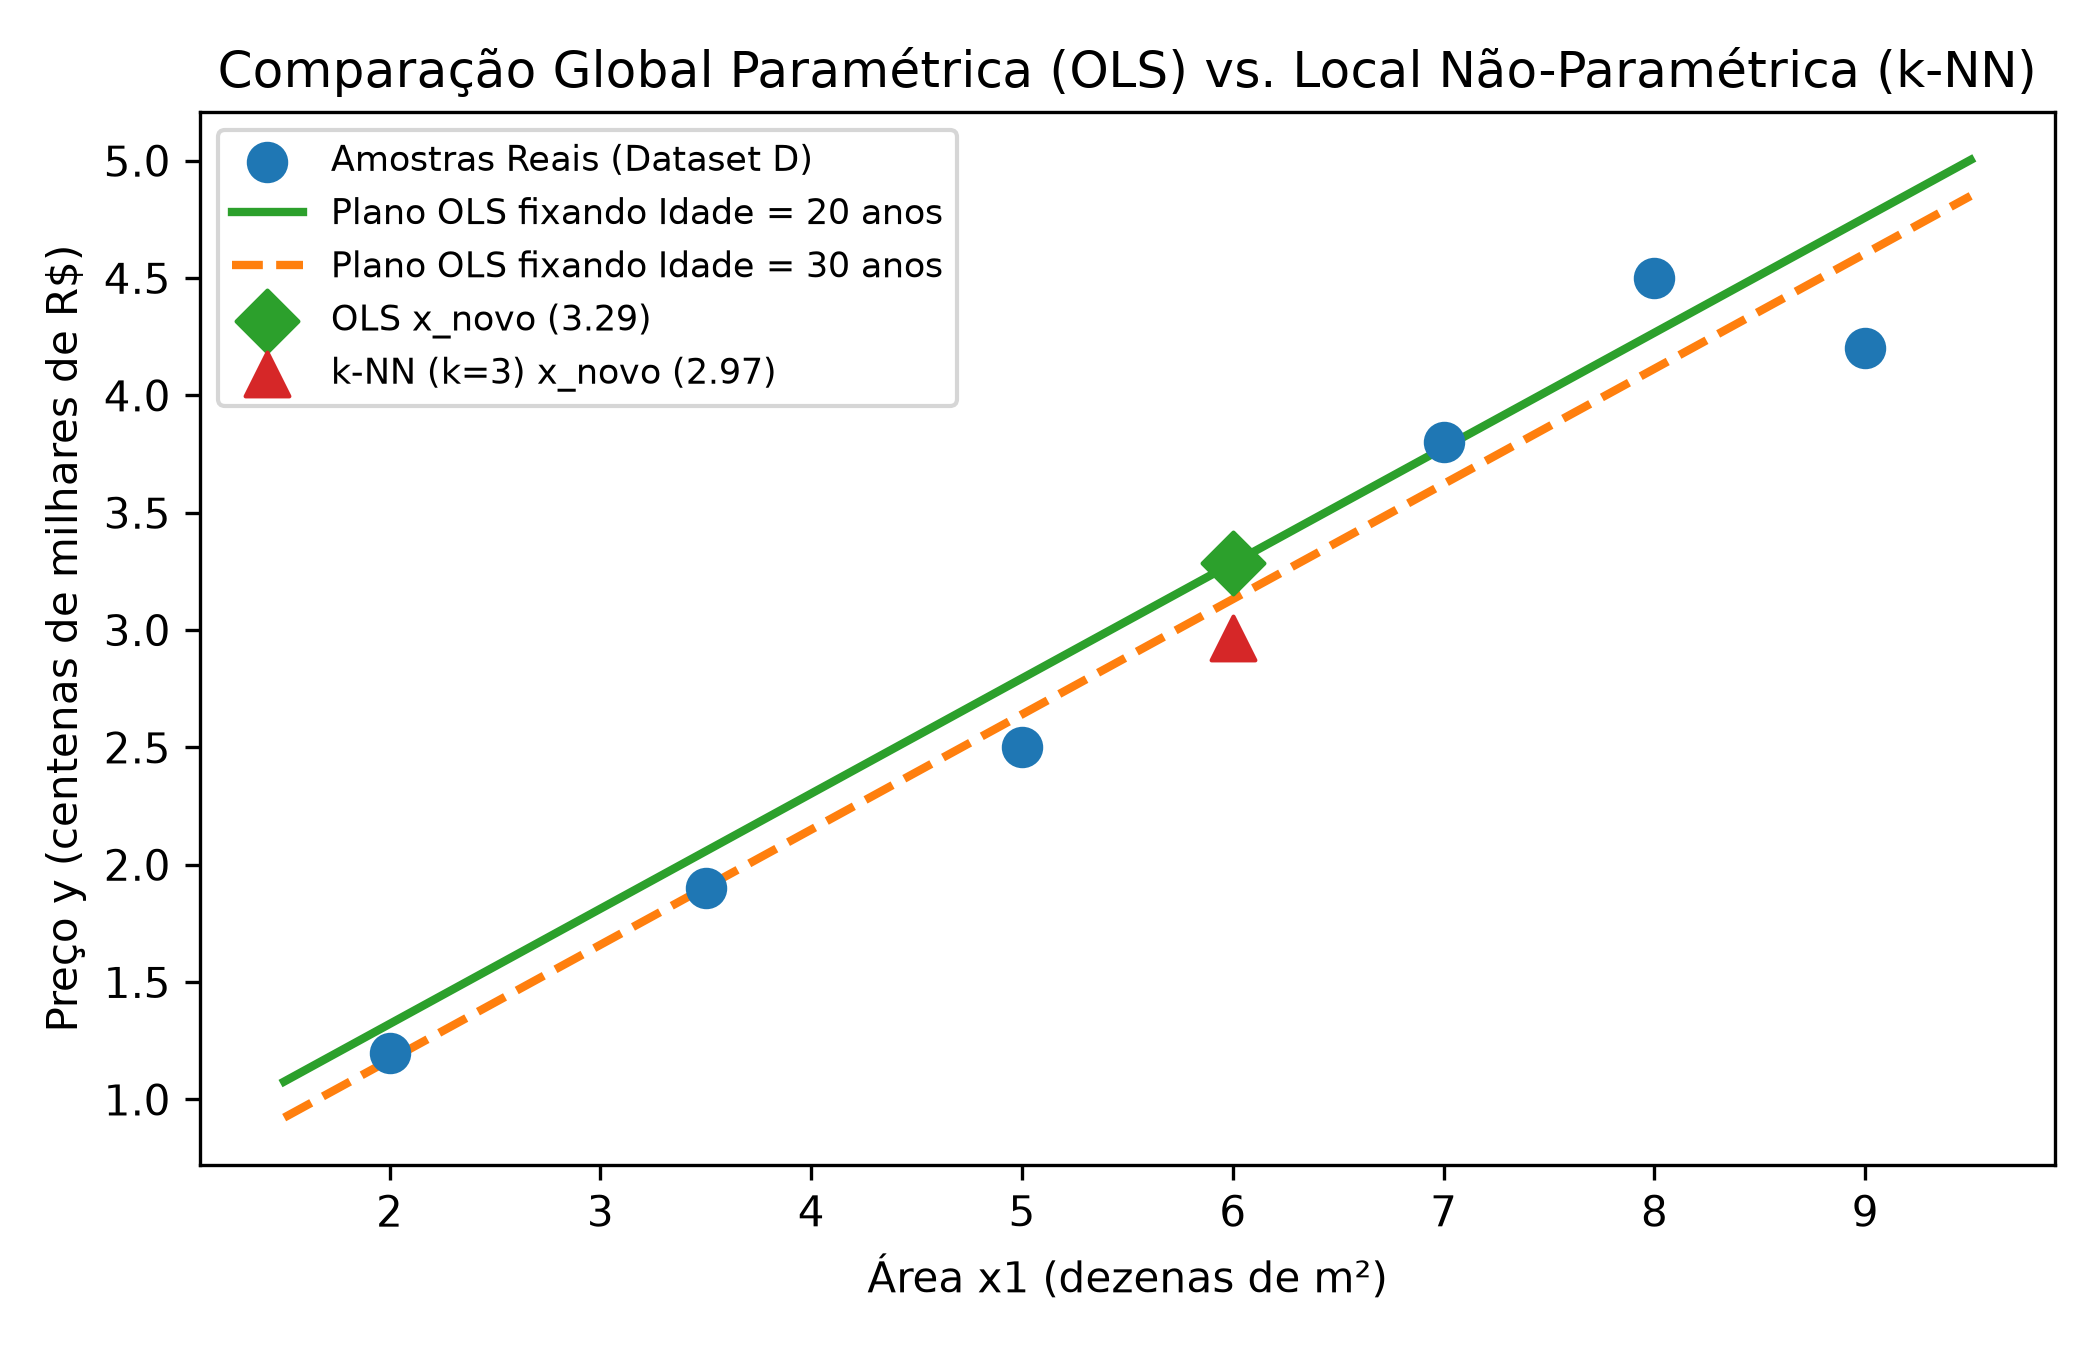
\includegraphics[width=0.80\textwidth]{../figures/q2_ols_vs_knn_superficie.png}
\caption{Comparação entre a regressão linear global (OLS) e a estimativa local ($k$-NN, $k=3$).}
\label{fig:q2}
\end{figure}

% ==============================================================================
\end{document}
